% ------------------------------------------------------------------------------
% The OpenQuake-engine Users Manual
%
% Authors:
%  Anirudh Rao       - GEM Foundation, Pavia, Italy
%	Marco Pagani 		- GEM Foundation, Pavia, Italy
% 	Vitor Silva 		- GEM Foundation, Pavia, Italy
%  Michele Simionato - GEM Foundation, Pavia, Italy
%	Robin Gee         - OGS, Trieste, Italy
%
% Authors on previous versions:
%  Helen Crowley     - GEM Foundation, Pavia, Italy
%  Damiano Monelli   - GEM Foundation, Pavia, Italy
%  Graeme Weatherill - GEM Foundation, Pavia, Italy
%
% License:
% Document distributed under the CC BY-NC-SA 4.0 License
% Creative Commons Attribution-NonCommercial-ShareAlike 4.0 International
% http://creativecommons.org/licenses/by-nc-sa/4.0/
%
% Copyright:
% © GEM Foundation, Pavia, Italy. 2013--2018.
% ------------------------------------------------------------------------------

%-------------------------------------------------------------------------------
%  PACKAGES AND OTHER DOCUMENT CONFIGURATIONS
%-------------------------------------------------------------------------------

\documentclass[11pt,fleqn]{book} % ------------------ Left-justified equations -
%%%%%%%%%%%%%%%%%%%%%%%%%%%%%%%%%%%%%%%%%%%%%%%%%%%%%%%%%%%%%%%%%%%%%%%%%%%%%%%%
% The GEM Technical Documentation LaTeX Template
% Version 1.0 (10/10/2015)
%
% Original author:
% Mathias Legrand (legrand.mathias@gmail.com)
%
% Adapted for use by the GEM Foundation by:
% James Brown (james.brown@globalquakemodel.org)
% Anirudh Rao (anirudh.rao@globalquakemodel.org)
%
% License:
% CC BY-NC-SA 3.0 (http://creativecommons.org/licenses/by-nc-sa/3.0/)
%
% Compiling this template:
% This template uses bibtex for its bibliography and makeindex for its index.
% When you first open the template, compile it from the command line with the
% commands below:
%
% 1) pdflatex -interaction=nonstopmode oq-manual.tex
% 2) bibtex oq-manual
% 3) pdflatex -interaction=nonstopmode oq-manual.tex
% 4) pdflatex -interaction=nonstopmode oq-manual.tex
% 5) makeindex oq-manual.idx
% 6) makeglossaries oq-manual
% 7) pdflatex -interaction=nonstopmode oq-manual.tex
%
% After this, when you wish to update the bibliography/index use the appropriate
% command above and make sure to compile with pdflatex several times
% afterwards to propagate your changes to the document.
%
% This template also uses a number of packages which may need to be updated
% to the newest versions for the template to compile. It is strongly
% recommended you update your LaTeX distribution if you have any
% compilation errors.
%
% Important note:
% Chapter heading images should have a 2:1 width:height ratio,
% e.g. 920px width and 460px height.
%
%%%%%%%%%%%%%%%%%%%%%%%%%%%%%%%%%%%%%%%%%%%%%%%%%%%%%%%%%%%%%%%%%%%%%%%%%%%%%%%%

%-------------------------------------------------------------------------------
%  PACKAGES AND OTHER DOCUMENT CONFIGURATION
%-------------------------------------------------------------------------------

% Page layout and margins
\usepackage[top=3cm,bottom=3cm,left=3.2cm,right=3.2cm,headsep=10pt,a4paper]{geometry}
\linespread{1.25}

% Page count
\usepackage{lastpage}

% Font settings
\usepackage[condensed]{roboto} % Use the Roboto font for headings
\usepackage[bitstream-charter]{mathdesign} % Use the Bitstream Charter font for text
% \usepackage{amsmath,amsfonts,amssymb,amsthm} % For math equations, theorems, symbols, etc
\usepackage{microtype} % Slightly tweak font spacing for aesthetics
\usepackage[utf8]{inputenc} % Required for including letters with accents
\usepackage[T1]{fontenc} % Use 8-bit encoding that has 256 glyphs

% Color settings
\usepackage{color, colortbl}
\usepackage{xcolor} % Required for specifying colors by name
\definecolor{darkgray}{gray}{.25}
\definecolor{lightgray}{gray}{.98}
% Colors from the GEM Brand Guidelines
\definecolor{oqblue}{RGB}{27,117,165}
\definecolor{gembrown}{cmyk}{.53,.54,.55,.54}

% Bibliography settings
\usepackage{csquotes}
\usepackage[style=alphabetic,
            sorting=nyt,
            sortcites=true,
            natbib=true,
            style=authoryear,
            maxcitenames=2,
            maxbibnames=100,
            autopunct=true,
            autolang=hyphen,
            hyperref=true,
            doi=true,
            abbreviate=false,
            backref=true,
            backend=bibtex,
            bibencoding=ascii,
            giveninits=true,
	    uniquename=false,
	    uniquelist=false]{biblatex}
\addbibresource{bibliography/hazard.bib} % Hazard BibTeX bibliography file
\addbibresource{bibliography/risk.bib} % Risk BibTeX bibliography file
\defbibheading{bibempty}{}

% Figure caption settings
\usepackage[textfont=it,margin=10pt,font=small,labelfont=bf,labelsep=endash]{caption}
\usepackage{subcaption}

% Rotate any object
\usepackage{rotating}

% Verbatim environments
\usepackage{verbatim}
\usepackage{fancyvrb}

% Index settings
\usepackage{calc} % Infix notation for \setcounter, \addtocounter, \setlength, \addtolength
\usepackage{imakeidx} % Required to make an index
\setcounter{secnumdepth}{3}
\setcounter{tocdepth}{3} % Entries down to \subsubsections in the TOC
\makeindex[title=Index,columns=2,intoc] % Create the files required for indexing

\usepackage{todonotes}
\usepackage{marginnote}
% Bold symbols in maths mode
\usepackage{bm}

% Flexible typesetting of tables and figures
\usepackage{ctable}
\usepackage{booktabs}

% Customization of section titles and table of contents
\usepackage{titlesec}
\usepackage{titletoc}

% Header and footer customization
\usepackage{fancyhdr}
\usepackage{etoolbox}

\usepackage{graphicx} % Required for including pictures
\usepackage{tikz} % Required for drawing custom shapes
\usepackage{eso-pic} % Required for specifying an image background in the title page
\usepackage{pdfpages} % Needed to load .pdf pages, used for the cover page

% English language hyphenation
\usepackage[english]{babel}

\usepackage{enumitem} % Customize lists
\setlist{nolistsep} % Reduce spacing between bullet points and numbered lists
\usepackage{listings} % Required for embedding code snippets
\usepackage[cache=true]{minted} % Syntax highlighting for xml

\usepackage{hyperref}
\hypersetup{
hidelinks,
colorlinks=true,
breaklinks=true,
citecolor=oqblue,
linkcolor=gembrown,
urlcolor=oqblue,
bookmarksopen=false,
pdftitle={The OpenQuake Engine Manual},
pdfauthor={GEM Foundation}
}

% Package to create a glossary - must be loaded after hyperref
\usepackage[acronym,nonumberlist,style=altlist,section=section,toc]{glossaries}
\makeglossaries


%----------------------------------------------------------------------------------------
%     MAIN TABLE OF CONTENTS
%----------------------------------------------------------------------------------------

% Remove the default margin
\contentsmargin{0cm}

% \titlecontents{section}
%                       [left]
%                       {above}
%                       {before with label}
%                       {before without label}
%                       {filler and page}
%                       [after]

% Part text styling
\titlecontents{part}
                    [0cm] % Indentation
                    {\addvspace{24pt}\Large\sffamily\bfseries} % Spacing and font options for parts
                    {\color{black!60}\contentslabel[\Large\thecontentslabel]{1.25cm}\color{black}} % Part number
                    {}
                    {\color{black!60}\Large\sffamily\bfseries\hfill\thecontentspage} % Page number
                    []

% Chapter text styling
\titlecontents{chapter}
                    [1.25cm] % Indentation
                    {\addvspace{18pt}\large\sffamily\bfseries} % Spacing and font options for chapters
                    {\color{darkgray!80}\contentslabel[\Large\thecontentslabel]{1.25cm}\color{darkgray}} % Chapter number
                    {\color{darkgray}}
                    {\color{darkgray!40}\large\sffamily\bfseries\;\titlerule*[.5pc]{.}\;\color{darkgray!80}\thecontentspage} % Page number
                    []

% Section text styling
\titlecontents{section}
                    [1.25cm] % Indentation
                    {\addvspace{12pt}\sffamily\bfseries} % Spacing and font options for sections
                    {\color{black!60}\contentslabel[\thecontentslabel]{1.25cm}\color{black}} % Section number
                    {}
                    {\color{black!20}\normalsize\sffamily\bfseries\;\titlerule*[.5pc]{.}\;\color{black!60}\thecontentspage} % Page number
                    []

% Subsection text styling
\titlecontents{subsection}
                    [1.25cm] % Indentation
                    {\addvspace{6pt}\sffamily\small} % Spacing and font options for subsections
                    {\color{black!60}\contentslabel[\thecontentslabel]{1.25cm}\color{black}} % Subsection number
                    {}
                    {\color{black!20}\normalsize\sffamily\;\titlerule*[.5pc]{.}\;\color{black!60}\thecontentspage} % Page number
                    []

% Subsubsection text styling
\titlecontents{subsubsection}
                    [1.25cm] % Indentation
                    {\addvspace{3pt}\sffamily\footnotesize} % Spacing and font options for subsubsections
                    {\color{black!60}\contentslabel[\thecontentslabel]{1.25cm}\color{black}\em} % Subsubsection number
                    {}
                    {\color{black!20}\normalsize\sffamily\;\titlerule*[.5pc]{.}\;\color{black!60}\thecontentspage} % Page number
                    []

%----------------------------------------------------------------------------------------
%     MINI TABLE OF CONTENTS IN CHAPTER HEADS
%----------------------------------------------------------------------------------------

% Section text styling
\titlecontents{lsection}[0em] % Indendation
{\footnotesize\sffamily} % Font settings
{}
{}
{}

% Subsection text styling
\titlecontents{lsubsection}[.5em] % Indentation
{\normalfont\footnotesize\sffamily} % Font settings
{}
{}
{}

%----------------------------------------------------------------------------------------
%     PAGE HEADERS
%----------------------------------------------------------------------------------------

% Patch fancyhdr to set the font and rule colors for headers and footers
\makeatletter
\patchcmd{\@fancyhead}{\rlap}{\color{oqblue}\rlap}{}{}
\patchcmd{\headrule}{\hrule}{\color{black}\hrule}{}{}
\patchcmd{\@fancyfoot}{\rlap}{\color{oqblue}\rlap}{}{}
\patchcmd{\footrule}{\hrule}{\color{black}\hrule}{}{}
\makeatother

\pagestyle{fancy}
\renewcommand{\chaptermark}[1]{\markboth{\sffamily\normalsize\bfseries\chaptername\ \thechapter.\ #1}{}} % Chapter text font settings
\renewcommand{\sectionmark}[1]{\markright{\sffamily\normalsize\thesection\hspace{5pt}#1}{}} % Section text font settings
\fancyhf{} \fancyhead[LE,RO]{\sffamily\normalsize\thepage} % Font setting for the page number in the header
\fancyhead[LO]{\rightmark} % Print the nearest section name on the left side of odd pages
\fancyhead[RE]{\leftmark} % Print the current chapter name on the right side of even pages
\renewcommand{\headrulewidth}{0.5pt} % Width of the rule under the header
\addtolength{\headheight}{7.5pt} % Increase the spacing around the header
\renewcommand{\footrulewidth}{0pt} % Removes the rule in the footer
\fancypagestyle{plain}{\fancyhead{}\renewcommand{\headrulewidth}{0pt}} % Style for when a plain pagestyle is specified

% Remove the header from odd empty pages at the end of chapters
\makeatletter
\renewcommand{\cleardoublepage}{
\clearpage\ifodd\c@page\else
\hbox{}
\vspace*{\fill}
\thispagestyle{empty}
\newpage
\fi}
\makeatother

%----------------------------------------------------------------------------------------
%     SECTION NUMBERING IN THE MARGIN
%----------------------------------------------------------------------------------------

\makeatletter
\renewcommand{\@seccntformat}[1]{\llap{\textcolor{oqblue}{\csname the#1\endcsname}\hspace{1em}}}
\renewcommand{\section}{\@startsection{section}{1}{\z@}
{-4ex \@plus -1ex \@minus -.4ex}
{1ex \@plus.2ex }
{\normalfont\large\sffamily\bfseries}}
\renewcommand{\subsection}{\@startsection {subsection}{2}{\z@}
{-3ex \@plus -0.1ex \@minus -.4ex}
{0.5ex \@plus.2ex }
{\normalfont\sffamily\bfseries}}
\renewcommand{\subsubsection}{\@startsection {subsubsection}{3}{\z@}
{-2ex \@plus -0.1ex \@minus -.2ex}
{.2ex \@plus.2ex }
{\normalfont\small\sffamily\bfseries}}
\renewcommand{\paragraph}{\@startsection {paragraph}{4}{\z@}
{-2ex \@plus-.2ex \@minus .2ex}
{.1ex}
{\normalfont\small\sffamily\bfseries\em}}
\makeatother

%----------------------------------------------------------------------------------------
%     PART HEADINGS
%----------------------------------------------------------------------------------------

% \titleformat{command}[shape]{format}{label}{sep}{before}[after]
\titleformat{\part}[display]{\bfseries\filcenter\Huge\sffamily}{\textcolor{gembrown}{\partname~\thepart}}{20pt}{\textcolor{gembrown}}

%----------------------------------------------------------------------------------------
%     CHAPTER HEADINGS
%----------------------------------------------------------------------------------------

% The set-up below should be manually adapted to the overall page
% layout and margin setup controlled by the geometry package.

\newcommand{\thechapterimage}{}
\newcommand{\chapterimage}[1]{\renewcommand{\thechapterimage}{#1}}

% Numbered chapters with mini tableofcontents
\makeatletter
\def\thechapter{\arabic{chapter}}
\def\@makechapterhead#1{
\thispagestyle{empty}
{\centering \normalfont\sffamily
\ifnum \c@secnumdepth >\m@ne
\if@mainmatter
\startcontents
\begin{tikzpicture}[remember picture,overlay]
\node at (current page.north west)
{\begin{tikzpicture}[remember picture,overlay]
\node[anchor=north west,inner sep=0pt] at (0,0) {\includegraphics[width=\paperwidth]{\thechapterimage}};

% Commenting the 3 lines below removes the small contents box in the chapter heading
\fill[color=oqblue!10!white,opacity=.6] (1cm,0) rectangle (12cm,-7cm);
\node[anchor=north west] at (1.5cm,.05cm) {\parbox[t][6.9cm][t]{10.5cm}{
    \huge\bfseries\flushleft \printcontents{l}{1}{\setcounter{tocdepth}{2}}}};
% The 3 lines below control the box environment for chapter titles
\draw[anchor=west] (1.8cm,-10cm) node [fill=white,text opacity=1,draw=white,draw opacity=1,line width=1.5pt,fill opacity=.6,inner sep=12pt]{\huge\sffamily\bfseries\textcolor{oqblue}{\thechapter.\hspace{0.35cm}#1\strut\makebox[22cm]{}}};

\end{tikzpicture}};
\end{tikzpicture}}
\par\vspace*{230\p@}
\fi
\fi}

% Unnumbered chapters without mini tableofcontents
\def\@makeschapterhead#1{
\thispagestyle{empty}
{\centering \normalfont\sffamily
\ifnum \c@secnumdepth >\m@ne
\if@mainmatter
\begin{tikzpicture}[remember picture,overlay]
\node at (current page.north west)
{\begin{tikzpicture}[remember picture,overlay]
\draw[anchor=west] (2.6cm,-4.2cm) node [fill=white,text opacity=1,draw=white,draw opacity=1,line width=1.5pt,fill opacity=.6,inner sep=12pt]{\huge\sffamily\bfseries\textcolor{oqblue}{#1\strut\makebox[22cm]{}}};
\end{tikzpicture}};
\end{tikzpicture}}
\par\vspace*{40\p@}
\fi
\fi
}
\makeatother
 % ------------- Load packages and template -
\graphicspath{{figures/}} % -------------- Directory where pictures are stored -

\begin{document}
% OpenQuake Book Glossary
% To cite a glossary element in a document:
%\gls{seismicsourcedata}
%\Gls{seismicsourcedata} - First initial is uppercase
%\GLS{seismicsourcedata} - All initials are uppercase
%\glspl{seismicsourcedata} - Plural
% To process the glossary:
% makeglossaries oq-manual


% ------- A

\newglossaryentry{areasource}{
	name=area source,
	description={A source type usually adopted to model distributed
	seismicity. In an area source the seismicity occurrence rate is assumed
	uniform over the source area; this produces an hazard pattern with a
	plateau of constant hazard inside the polygon delimiting the area source
	and values of hazard that tend to decrease as we move away from the
	border of the source}
}


\newglossaryentry{asset}{
	name=asset,
	description={An asset is an element with a certain value, which can include
	buildings or population. For example, an asset can include an individual
	building at a given location, or a number of buildings that are grouped, co-
	located at a single location and classified with the same \gls{taxonomy}}
}



% ------- B

\newglossaryentry{branch}{
	name=branch,
	plural=branches,
	description={The simplest element in a logic tree; it belongs to a
	\gls{branchset} where it represents one possible option among a finite
	number of alternatives. A branch is associated with a weight value if the \gls{branchset} represents the epistemic
	uncertainty on a parameter or a model when the \gls{branchset} is used to
	specify alternative models (e.g. district \glspl{acr:mfd})}
}


\newglossaryentry{branchinglevel}{
	name=branching level,
	description={It indicates the position where a \gls{branchset} or a
	\gls{branch} is located in a logic tree structure. For example, the first
	branching level of the \gls{seismicsourcelogictree} always contains one
	or several \glspl{initialseismicsourceinputmodel}}
}


\newglossaryentry{branchset}{
	name=branch set,
	description={The structure describing the epistemic uncertainty on a
	specific parameter or model included in a logic tree structure. It
	ensembles a number of \glspl{branch}, each one representing a discrete
	alternative}
}



% ------- C

\newacronym{cpsha}{cPSHA}{Classical PSHA}


\newglossaryentry{configurationfile}{
	name=configuration file,
	description={The file (usually .ini) containing the information necessary to
	run a calculation in OpenQuake}
}


\newglossaryentry{consequencefunction}{
	name=consequence function,
	description={the distribution of the consequence (or loss) ratio conditional
	on a set of discrete limit states, defined for a particular \gls{taxonomy}}
}


\newglossaryentry{consequencemodel}{
	name=consequence model,
	description={A set of \glspl{consequencefunction} used to model the
	consequence ratios of all the \glspl{taxonomy} in the \gls{exposuremodel}}
}


\newglossaryentry{charfaultsource}{
	name=characteristic fault source,
	description={A fault source typology where ruptures always cover the entire
	fault surface}
}


\newglossaryentry{complexfaultsource}{
	name=complex fault source,
	description={A source typology usually adopted to model subduction
	interface faults}
}



% ------- D

\newglossaryentry{deductible}{
	name=deductible,
	description={A parameter used in the calculation of insured losses that
	establishes the economic value that needs to be deducted from the ground-up
	losses}
}


\newglossaryentry{seismichazarddisaggregation}{
	name=seismic hazard disaggregation,
	description={A methodology to investigate the contributions to a
	specific level of hazard in terms of fundamental variables commonly used
	to characterize seismic sources and ground motion models (e.g. magnitude,
	source-site distance, \gls{epsilon}}
}


\newglossaryentry{dip}{
	name=dip,
	description={The dip is the steepest angle of descent of the fault plane
	relative to a horizontal plane; it is measured in degrees [0,90]}
}


\newglossaryentry{disaggregationmatrix}{
	name=disaggregation matrix,
	description={A multi-dimensional matrix used to systematically store the
	contributions to a level of hazard to be disaggregated and that is specified
	by the user. See also \gls{seismichazarddisaggregation}}
}



% ------- E

\newacronym{acr:erf}{ERF}{Earthquake\- Rupture\- Forecast}
\newacronym{acr:epsha}{ePSHA}{Event-based PSHA}


\newglossaryentry{earthquakeruptureforecast}{
	name=earthquake rupture forecast,
	description={A list of all possible ruptures generated by all the
	sources included in a seismic source model. Each element in the list
	contains: the rupture geometry and the rupture probability of occurrence
	in a given time span. See also the definition available on the
	\href{http://www.opensha.org/glossary-earthquakeRuptureForecast} {OpenSHA
	website}}
}


\newglossaryentry{earthquakeruptureforecastcalculator}{
	name=earthquake rupture forecast calculator,
	description={Calculator producing a \gls{seismicsourcemodel} from a
	\gls{seismicsourcelogictree}}
}


\newglossaryentry{epsilon}{
	name=epsilon,
	description={normalized residual of the ground motion}
}


\newglossaryentry{exposuremodel}{
	name=exposure model,
	description={A set of \glspl{asset} grouped according to their
	geographical location, \gls{taxonomy} and value}
}



% ------- F

\newglossaryentry{faulttrace}{
	name=fault trace,
	description={A curve representing the intersection between the surface
	containing the fault surface (or its prolongation) and the topographic
	surface
	\begin{figure}[!ht] \centering
	\includegraphics[width=10cm]{figures/hazard/single_rupture.pdf}
	\end{figure}}
}


\newglossaryentry{fragilityfunction}{
	name=fragility function,
	description={the probability of exceeding a set of limit states, given
	an intensity measure level. These functions can be discrete or continuous}
}


\newglossaryentry{fragilitymodel}{
	name=fragility model,
	description={A set of \glspl{vulnerabilityfunction} used to model the
	fragility of all the \glspl{asset} in the \gls{exposuremodel}}
}


\newglossaryentry{frequencymagnitudedistribution}{
	name=frequency-magnitude distribution,
	description={See \gls{mfd}}
}



% ------- G

\newacronym{acr:gem}{GEM}{Global Earthquake Model}
\newacronym{acr:gmf}{GMF}{Ground Motion Field}
\newacronym{acr:gmpe}{GMPE}{Ground Motion Prediction Equation}
\newacronym{acr:gmlt}{GMLT}{Ground Motion Logic Tree (see \gls{groundmotionlogictree}}


\newglossaryentry{gridsource}{
	name=grid source,
	description={A source typology usually adopted to model distributed
	seismicity. It is routinely produced by a seismicity smoothing algorithm (one
	of the most famous algorithm is the one proposed by \citet{frankel1995})}
}


\newglossaryentry{groundmotionfield}{
	name=ground-motion field,
	description={An object describing the geographic distribution around a
	rupture of a ground motion intensity measure}
}


\newglossaryentry{groundmotionfieldcalc}{
	name=ground-motion field calculator,
	description={An \gls{acr:oqe} calculator that given a rupture computes the
	geographic distribution of a ground motion intensity parameter. Currently
	OQ can generate ground motion fields using a \gls{acr:gmpe}}
}


\newglossaryentry{groundmotionlogictree}{
	name=ground-motion logic tree,
	description={A method used to systematically describe the epistemic
	uncertainties related to the ground motion models used in the computation
	of hazard using a specific \gls{pshainputmodel}}
}


\newglossaryentry{groundmotionmodel}{
	name=ground-motion model,
	description={An object that given a rupture with specific properties
	computes the expected ground motion at the given site. In simplest case a
	ground motion model corresponds to a \gls{groundmotionpredictioneq}. In
	case of complex PSHA input models, the produced ground motion models
	contains a set of \glspl{acr:gmpe}, one for each tectonic region considered}
}


\newglossaryentry{groundmotionparameter}{
	name=ground-motion parameter,
	description={A scalar or vector quantity describing a relevant property
	of the shaking such as intensity (e.g. PGA or Spectral Acceleration)
	or duration, equivalent number of cycles  \citep[see for
	example][]{hancock2005})}
}


\newglossaryentry{groundmotionpredictioneq}{
	name=ground-motion prediction equation,
	description={An equation that - given some fundamental parameters
	characterizing  the source, the propagation path and the site (in the
	simplest  case magnitude, distance and V$_\text{S,30}$) - computes the
	value $GM$ of a (scalar) ground motion intensity parameter}
}


\newglossaryentry{groundmotionsystem}{
	name=ground-motion system,
	description={An object containing a list of \gls{groundmotionlogictree}}
}



% ------- I

\newglossaryentry{initialseismicsourceinputmodel}{
	name=initial seismic source input model,
	description={It is the ensable of information needed to fully describe
	the seismic sources composing a seismic source input model. The
	initial seismic source input model is included in the first branching
	level of a seismic source logic tree}
}


\newglossaryentry{insuredlosses}{
	name=insured losses,
	description={Fraction of the ground-up losses that can be covered by the
	insurance industry, according to a certain policy}
}

\newacronym{acr:irmt}{IRMT}{}
\newglossaryentry{irmt}{
	name=Integrated Risk Modelling Toolkit,
	description={A plugin for QGIS which includes tools to run the \gls{oqe},
	to visualize hazard and risk results, to develop composite indicators
	and integrate them with physical risk estimations, and to predict building
	recovery times following an earthquake.
	This plugin was designed as a collaborative effort between the
	GEM Foundation and the Center for Disaster Management and Risk Reduction
	Technology, and it has been developed by the GEM Foundation.}
}

\newglossaryentry{investigationtime}{
	name=investigation time,
	description={The time interval considered to calculate hazard; usually
	it corresponds to 50 years}
}



% ------- L

\newglossaryentry{limit}{
	name=limit,
	description={A parameter used in the calculation of insured losses that
	establishes the maximum economic amount that can be covered by the insurance
	industry, according to a certain insurance policy}
}


\newglossaryentry{logictree}{
	name=logic tree,
	description={Data structure used to systematically describe uncertainties
	on parameters and models used in a PSHA study}
}


\newglossaryentry{logictreeprocessor}{
	name=logic tree processor,
	description={An OQ calculator that takes the PSHA Input Model and creates
	many realisations of a \gls{seismicsourcemodel} and of a
	\gls{groundmotionmodel}}
}


\newacronym{acr:ltmcs}{LTMCS}{Logic Tree Monte Carlo Sampler}

%------------M

\newglossaryentry{msr}{
	name=magnitude-scaling relationship,
	description={An empirical relationship linking the magnitude with a
	parameter  describing the size of the corresponding rupture (e.g. the
	area  of the rupture or the rupture length)}
}


\newacronym{acr:mfd}{MFD}{Magnitude-Frequency Distribution}
\newglossaryentry{mfd}{
	name=magnitude-frequency distribution,
	description={A distribution describing the frequency of earthquakes with
	a specific magnitude. It can be continuous or discrete. One frequency-
	magnitude distribution frequently adopted in \gls{acr:psha} is the double
	truncated Gutenberg-Richter distribution}
}

%---------------N
\newglossaryentry{nonparametricsource}{
    name=non-parametric source,
    description={A source typology in which the earthquake rupture forecast is
    described explicitly by a set of ruptures and the corresponding
    probabilities of occurrence}
}



% ------- N

\newacronym{acr:nrml}{NRML}{Natural hazards' Risk Markup Language}
\newglossaryentry{nrml}{
	name=Natural hazards' Risk Markup Language,
	description={A markup language similar to XML, which specifies a number
	of standardised schemas to represent various input models used for
	\gls{acr:oqe} calculations and output files generated by \gls{acr:oqe}
	calculations
	}
}



% ------- O

\newacronym{acr:hazlib}{oq-hazardlib}{OpenQuake hazard library}


\newglossaryentry{opensha}{
	name=OpenSHA,
	description={OpenSHA is an open-source, advanced Java-based platform
	for conducting Seismic Hazard Analysis - (see
	\href{http://opensha.org}{OpenSHA website})}
}


\newacronym{acr:oqe}{oq-engine}{OpenQuake-engine}
\newacronym{acr:oqe17}{oq-engine 1.7}{OpenQuake-engine v1.7}
\newacronym{acr:oqe18}{oq-engine 1.8}{OpenQuake-engine v1.8}
\newacronym{acr:oqe19}{oq-engine 1.9}{OpenQuake-engine v1.9}
\newacronym{acr:oqe20}{oq-engine 2.0}{OpenQuake-engine v2.0}
\newacronym{acr:oqe21}{oq-engine 2.1}{OpenQuake-engine v2.1}
\newacronym{acr:oqe22}{oq-engine 2.2}{OpenQuake-engine v2.2}
\newacronym{acr:oqe23}{oq-engine 2.3}{OpenQuake-engine v2.3}
\newacronym{acr:oqe24}{oq-engine 2.4}{OpenQuake-engine v2.4}
\newacronym{acr:oqe25}{oq-engine 2.5}{OpenQuake-engine v2.5}
\newacronym{acr:oqe26}{oq-engine 2.6}{OpenQuake-engine v2.6}
\newacronym{acr:oqe27}{oq-engine 2.7}{OpenQuake-engine v2.7}
\newacronym{acr:oqe28}{oq-engine 2.8}{OpenQuake-engine v2.8}
\newacronym{acr:oqe29}{oq-engine 2.9}{OpenQuake-engine v2.9}



% ------- P

\newacronym{acr:pga}{PGA}{Peak Ground Acceleration}
\newacronym{acr:pgv}{PGV}{Peak Ground Velocity}

\newacronym[description={\glslink{psha}{Probabilistic Seismic Hazard
	Analysis}}]{acr:psha}{PSHA}{Probabilistic Seismic Hazard Analysis}


\newglossaryentry{pointsource}{
	name=point source,
	description={The elemental source typology used in the \glsdesc{acr:oqe} to
	model distributed seismicity}
}


\newglossaryentry{pshainputmodel}{
	name=PSHA input model,
	description={An object containing the information necessary to describe
	the seismic source and the ground motion models - plus the related
	epistemic uncertainties}
}


\newglossaryentry{psha}{
	name=probabilistic seismic hazard analysis,
	description={A methodology to compute seismic hazard by taking into
	account the potential contributions coming from all the sources of
	engineering importance for a specified site}
}



% ------- R

\newacronym{acr:risklib}{oq-risklib}{OpenQuake risk library}


\newacronym{acr:rrup}{$\text{r}_{\text{rup}}$}{closest distance between the
	site and rupture}


\newglossaryentry{rupture}{
	name=earthquake rupture,
	description={A 3D surface - representing a portion or the entire fault
	surface - over which a slip event (i.e. an earthquake) occurs}
}


\newglossaryentry{rupturemodel}{
	name=rupture model,
	description={An object containing the information necessary to describe
	a \gls{rupture}, such as magnitude, hypocenter location, strike, dip, 
	rake, and seismogenic depths}
}


\newglossaryentry{ruptureaspectratio}{
	name=rupture aspect ratio,
	description={The ratio between the lenght and the width of an
	earthquake rupture}
}


\newglossaryentry{rake}{
	name=rake,
	description={The rake is the direction in which a hanging wall block moves
	during a rupture, measured relative to fault strike on the plane of the
	fault}
}



% ------- S

\newacronym{acr:ssha}{SSHA}{Scenario Based Seismic Hazard Analysis}


\newglossaryentry{scenariohazard}{
	name=scenario based seismic hazard analysis,
	plural=scenario based seismic hazard analyses,
	description={An analyis of seismic hazard based on the selection of
	one or a few ruptures and the computation of the expected ground
	motion at a set of sites using a \gls{gmpe} accounting ground motion
	variability}
}


\newglossaryentry{seismicityhistory}{
	name=seismicity history,
	plural=seismicity histories,
	description={An object containing a set ruptures representative of the
	possible seismicity generated by the sources in a
	\gls{seismicsourcemodel} during the investigation time $t$}
}


\newglossaryentry{seismicityrate}{
	name=seismicity rate,
	description={Number of events per unit of time (if not better
	specified, the definition of a seismicity rate generally presumes a time
	independent}
}


\newglossaryentry{seismicsourcedata}{
	name=seismic source data,
	description={An object containing the information necessary to
	completely describe a \gls{acr:psha} seismic source i.e. seismic source
	type, position, geometry and seismicity occurrence model}
}


\newglossaryentry{seismicsourcelogictree}{
	name=seismic source logic tree,
	description={Logic tree structure defined to describe in structured and
	systematic way the epistemic uncertainties characterizing the seismic
	source model. The first branching level in the logic tree by definition
	contains one or several alternative \gls{initialseismicsourceinputmodel}}
}


\newacronym{acr:ssim}{SSIM}{Seismic Source Input Model}


\newglossaryentry{seismicsourceinputmodel}{
	name=seismic source input model,
	description={An object containing a list of \gls{seismicsourcedata}. In
	the \glsdesc{acr:oqe} a seismic source model doesn't contain epistemic
	uncertainty}
}


\newglossaryentry{seismicsource}{
	name=seismic source,
	description={An object that can generate}}


\newacronym{acr:ssm}{SSM}{Seismic Source Model}
\newglossaryentry{seismicsourcemodel}{
	name=seismic source model,
	description={An object containing a list of \glspl{seismicsource}
	objects}
}


\newacronym{acr:scec}{SCEC}{Southern California Earthquake Center}


\newglossaryentry{seismicsourcesystem}{
	name=seismic source system,
	description={An object containing a list of
	\glspl{initialseismicsourceinputmodel} and the
	\gls{seismicsourcelogictree}}
}


\newglossaryentry{simplefaultsource}{
	name=simple fault source,
	description={A source typology usually adopted to model shallow
	structures with an uncomplicated geometry}
}


\newacronym{acr:ses}{SES}{Stochastic Event Set}
\newglossaryentry{stochasticeventset}{
	name=stochastic event set,
	description={An object containing one or many \glspl{seismicityhistory}}
}


\newglossaryentry{strike}{
	name=strike,
	description={The strike direction correspond to the angle between the
	north and the direction you take so that when you walk along the
	\gls{faulttrace} the fault dips on your right}
}


\newacronym{acr:sa}{S$_a$}{Spectral Acceleration}



% ------- T

\newglossaryentry{tag}{
	name=tag,
	plural=tags,
	description={Scheme used to specify attributes for the \glspl{asset}.
	Attributes for an \gls{asset} could include the state, county, zip-code,
	city, occupancy, CRESTA ID, or other such markers that could be used 
	in the post-processing stage of a risk calculation to aggregate
	results for each tag.}
}

\newglossaryentry{taxonomy}{
	name=taxonomy,
	plural=taxonomies,
	description={Scheme used to classify the \glspl{asset}. For buildings, a
	classification scheme has been proposed by \gls{acr:gem} which considers a
	number of attributes including lateral load resisting system and its
	material, height, year of construction. The taxonomy is currently used to
	link the \glspl{asset} in the \gls{exposuremodel} to the relevant
	\gls{vulnerabilityfunction} or \gls{fragilityfunction}}
}


\newglossaryentry{tectonicregion}{
	name=tectonic region,
	description={A area on the topographic surface that can be considered
	homogeneous in terms of tectonic properties such as the prevalent
	seismogenic properties and/or the seismic wave propagation properties}
}


\newglossaryentry{temporaloccurrencemodel}{
	name=temporal occurrence model,
	description={Usually a probabilistic model giving the probability of
	occurrence of an event in a specified \gls{investigationtime}}
}



% ------- U

\newacronym{acr:usgs}{USGS}{United States Geological Survey}



% ------- V

\newglossaryentry{vulnerabilityfunction}{
	name=vulnerability function,
	description={A function that describes the probability distribution of
	loss ratio, conditioned on an intensity measure level. Currently only
	discrete vulnerability functions are supported}
}


\newglossaryentry{vulnerabilitymodel}{
	name=vulnerability model,
	description={A set of \glspl{vulnerabilityfunction} used to model the
	physical vulnerability of all the \glspl{asset} in the \gls{exposuremodel}}
}


\newglossaryentry{acr:vs30}{
	name=V$_{S,30}$,
	description={Average shear wave velocity of the materials in the uppermost
	30m of the soil column}
}
 % ---------------------------------------- Load glossary -

%-------------------------------------------------------------------------------
%  COVER PAGE
%-------------------------------------------------------------------------------

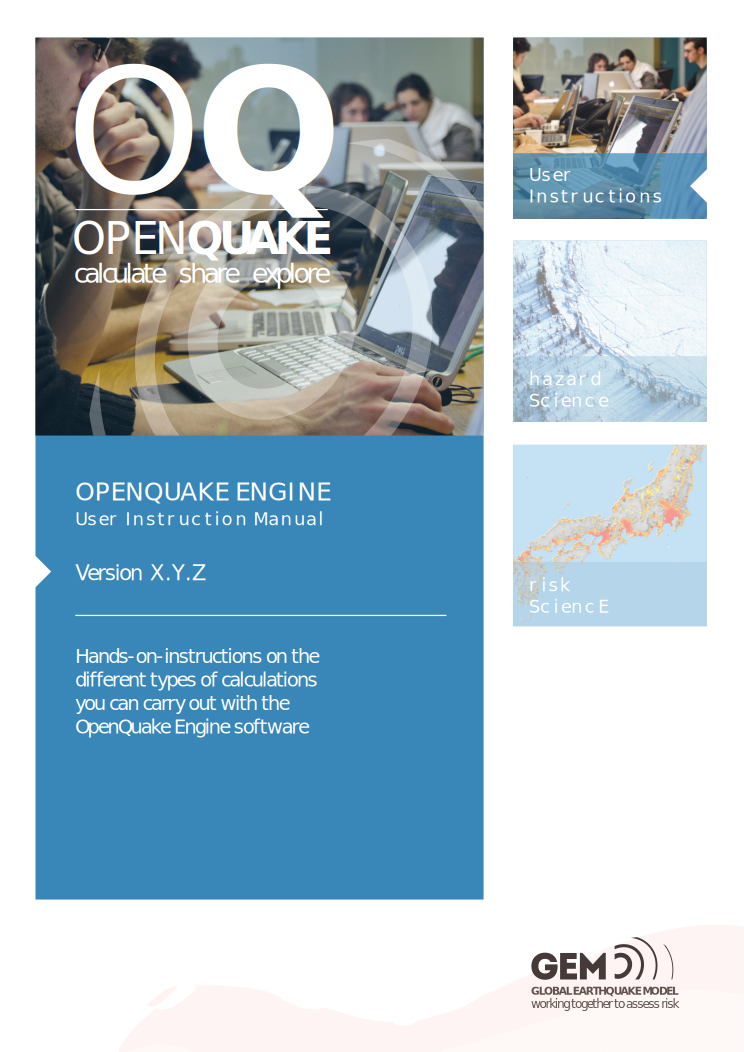
\includepdf[pages=-]{figures/oq_manual_cover.pdf}

%-------------------------------------------------------------------------------
%  TITLE PAGE
%-------------------------------------------------------------------------------

\begingroup
\thispagestyle{empty}
\begin{center}
\par\normalfont\fontsize{15}{15}\sffamily\selectfont
\textcolor{oqblue}{OpenQuake: calculate, share, explore}
\vspace*{9cm}
\par\bfseries\fontsize{35}{35}\sffamily\selectfont
\textcolor{gembrown}{The OpenQuake-engine\\User Instruction Manual}\par
\vspace*{9cm}
\par\normalfont\fontsize{15}{15}\sffamily\selectfont
\href{http://globalquakemodel.org/openquake/}{\textcolor{oqblue}{globalquakemodel.org/openquake}}
\end{center}
\endgroup

%-------------------------------------------------------------------------------
%  COPYRIGHT PAGE
%-------------------------------------------------------------------------------

\newpage
~\vfill
\thispagestyle{empty}

\noindent
   \textbf{Authors} \\
   Marco Pagani$^1$, Vitor Silva$^1$,
   Anirudh Rao$^1$, Michele Simionato$^1$, Robin Gee$^1$\hfill \\
   \hfill \\
   \textbf{Authors on previous versions} \\
   Helen Crowley$^2$, Damiano Monelli, Graeme Weatherill$^3$\hfill \\
   \hfill \\
   \small
   \begin{tabular}{p{4cm}p{4cm}p{4cm}}
   $^1$ GEM Foundation \hfill \newline
   via Ferrata, 1 \hfill \newline
   20133 Pavia \hfill \newline
   Italy \hfill \newline
   &
   $^2$ EUCENTRE \hfill \newline
   via Ferrata, 1 \hfill \newline
   20133 Pavia \hfill \newline
   Italy \hfill \newline
   &
   $^3$ GFZ \hfill \newline
   Helmholtzstraße 6/7 \hfill \newline
   14467 Potsdam \hfill \newline
   Germany \hfill \newline
   \end{tabular} \hfill \newline
   %
   Email address for all current authors:\hfill\\
   $<$name.surname$>$@globalquakemodel.org\hfill\\
   \normalsize

\noindent
   {\textbf{Citation}} \hfill \\
   Please cite this document as: \hfill \\
   GEM (#PUBYEAR#). The OpenQuake-engine User Manual.
   \textit{Global Earthquake Model (GEM) OpenQuake Manual for Engine version X.Y.Z.\\
   doi: 10.13117/GEM.OPENQUAKE.MAN.ENGINE.X.Y.Z, \pageref{LastPage} pages.} \hfill \\
\noindent \hfill\\
\noindent
   {\bf{Disclaimer}} \hfill \\
   The OpenQuake-engine User Manual is distributed in the hope that it will be
   useful, but without any warranty: without even the implied warranty of
   merchantability or fitness for a particular purpose. While every precaution
   has been taken in the preparation of this document, in no event shall the
   authors of the Manual and the GEM Foundation be liable to any party for
   direct, indirect, special, incidental, or consequential damages, including
   lost profits, arising out of the use of information contained in this
   document or from the use of programs and source code that may accompany it,
   even if the authors and GEM Foundation have been advised of the possibility
   of such damage. The Manual provided hereunder is on as ``as is'' basis, and
   the  authors and GEM Foundation have no obligations to provide maintenance,
   support, updates, enhancements, or modifications. \hfill \\
\noindent \hfill\\
\noindent
   {\bf{License}} \hfill \\
   This Manual is distributed under the Creative Commons License  Attribution-
   NonCommercial-ShareAlike 4.0 International
   (\href{http://creativecommons.org/licenses/by-nc-sa/4.0/} {CC BY-NC-SA
   4.0}). You can download this Manual and share it with others as long as you
   provide proper credit, but you cannot change it in any way or use it
   commercially.\hfill \\

\noindent \copyright\ \textsc{2013--#PUBYEAR# GEM Foundation}\\
\noindent \textit{#PUBMONTH# #PUBYEAR#} % Printing/edition date

%-------------------------------------------------------------------------------
%  TABLE OF CONTENTS
%-------------------------------------------------------------------------------

\chapterimage{figures/chapter_head.pdf} % Table of contents heading image
\pagestyle{empty} % No headers
\tableofcontents % Print the table of contents itself
\cleardoublepage % Forces the first chapter to start on the right
\pagestyle{fancy} % Print headers again

%-------------------------------------------------------------------------------
%  FOREWORD
%-------------------------------------------------------------------------------
\chapterimage{figures/chapter_head.pdf} % Chapter heading image
\chapter*{Preface}
\addcontentsline{toc}{chapter}{Preface}
\input{oqum/preamble}

%-------------------------------------------------------------------------------
%  THE MANUAL
%-------------------------------------------------------------------------------

% ------------------------------------------------------- Part I: Introduction -
\part{Introduction}
\label{part:introduction}
\chapterimage{figures/chapter_head.pdf} % Chapter heading image
\chapter{OpenQuake-engine Background}
   \label{chap:intro}
	\input{oqum/introduction}

% ----------------------------------------------------- Part II: Hazard Module -
\thispagestyle{empty}
\part{Hazard}

\chapterimage{figures/chapter_head.pdf} % Chapter heading image
\chapter{Introduction to the Hazard Module}
   \label{chap:hazintro}
	\index{OpenQuake-engine!Hazard}

The hazard component of the \glsdesc{acr:oqe} builds on top of the
\gls{acr:hazlib}, a Python-based library containing tools for PSHA
calculations.

The web repository of this library is available at the following address:\\
\href{https://github.com/gem/oq-engine/tree/master/openquake/hazardlib}{https://github.com/gem/oq-engine/tree/master/openquake/hazardlib}.

In this section we briefly illustrate the main properties of the hazard
component of the \glsdesc{acr:oqe}. In particular, we will describe the main
typologies of sources supported and the main calculation workflows available.


\section{Source typologies}
\index{Source type}
\label{sec:source_typologies}
\input{oqum/hazard/00a_source_typologies}

\section{Magnitude-frequency distributions}
\label{sec:mfd_list}
\input{oqum/hazard/00b_mfds}

\section{Magnitude-scaling relationships}
\label{sec:msr_list}
We provide below a list of the magnitude-area scaling relationships
implemented in the \gls{acr:hazlib}:

\subsection{Relationships for shallow earthquakes in active tectonic regions}

\begin{itemize}

    \item \cite{wells1994} - One of the most well known magnitude scaling
	relationships, based on a global database of historical earthquake
	ruptures. The implemented relationship is the one linking magnitude to
	rupture area, and is called with the keyword \verb=WC1994=

\end{itemize}


\subsection{Magnitude-scaling relationships for subduction earthquakes}
\begin{itemize}
    \item \cite{Strasser2010} - Defines several magnitude scaling relationships for interface and in-slab earthquakes. Only the magnitude to rupture-area scaling relationships are implemented here, and are called with the keywords \verb=StrasserInterface= and \verb=StrasserIntraslab= respectively.
    \item \cite{Thingbaijam2017} - Define  magnitude scaling relationships for interface. Only the magnitude to rupture-area scaling relationships are implemented here, and are called with the keywords \verb=ThingbaijamInterface=.
\end{itemize}

\subsection{Magnitude-scaling relationships stable continental regions}
\begin{itemize}
    \item \cite{ceus2011} - Defines a single magnitude to rupture-area scaling relationship for use in the central and eastern United States: $Area = 10.0^{M_W - 4.336}$. It is called with the keyword \verb=CEUS2011=
\end{itemize}

\subsection{Miscellaneous Magnitude-Scaling Relationships}
\begin{itemize}
    \item \verb=PeerMSR= defines a simple magnitude scaling relation used as part of the Pacific Earthquake Engineering Research Center verification of probabilistic seismic hazard analysis programs: $Area = 10.0 ^{M_W - 4.0}$.
    \item \verb=PointMSR= approximates a `point' source by returning an infinitesimally small area for all magnitudes. Should only be used for distributed seismicity sources and not for fault sources. 
\end{itemize}

%
%\subsection{Ground motion prediction equations for volcanic areas}
%\begin{itemize}
%    \item
%\end{itemize}


\section{Calculation workflows}
\index{OpenQuake-engine!Hazard calculation workflows}
\label{sec:hazard_calculators}
\input{oqum/hazard/00d_hazard_workflows}
   \cleardoublepage

\chapterimage{figures/chapter_head.pdf} % Chapter heading image
\chapter{Using the Hazard Module}
	\label{chap:hazinputs}
	This Chapter summarises the structure of the information necessary to define
a PSHA input model to be used with the \glsdesc{acr:oqe}.

Input data for probabilistic based seismic hazard analysis (Classical, Event
based, Disaggregation, and Uniform Hazard Spectra) are organised into:

\begin{itemize}

	\item A general configuration file.

    \item A file describing the Seismic Source System, that is the set of
	initial source models and associated epistemic uncertainties needed to
	model the seismic activity in the region of interest.

    \item A file describing the Ground Motion System, that is the set of
	ground motion prediction equations, per tectonic region type, needed to
	model the ground motion shaking in the region of interest.

\end{itemize}

Figure~\ref{fig:psha_input} summarises the structure of a PSHA input model
for the \glsdesc{acr:oqe} and the relationships between the different files.

\begin{figure}[!ht]
\centering
\includegraphics[width=14cm]{figures/hazard/psha_input_structure.pdf}
\caption{PSHA Input Model structure}
\label{fig:psha_input}
\end{figure}


\section{Defining Logic Trees}
\input{oqum/hazard/01a_logic_trees.tex}
\label{sec:hazard_logic_trees}

\section{The Seismic Source System}
\input{oqum/hazard/01b_seismic_source_system}
\label{sec:seismic_source_system}

\section{The Ground Motion System}
\index{Input!Ground motion system}
\label{sec:ground_motion_system}
\input{oqum/hazard/01c_ground_motion_system}

\section{Configuration file}
\index{Input!Configuration file!Hazard}
\label{sec:hazard_configuration_file}
\input{oqum/hazard/01d_config.tex}
   \cleardoublepage

\chapterimage{figures/chapter_head.pdf} % Chapter heading image
\chapter{Hazard Calculations and Results}
	\label{chap:hazoutputs}
	In this Chapter we provide a desciption of the main commands available for
running hazard with the \gls{acr:oqe} and the file formats used to represent
the results of the analyses.

A general introduction on the use of the \glsdesc{acr:oqe} is provided in
Chapter~\ref{chap:intro} at page~\pageref{chap:intro}. The
reader is invited to consult this part before diving into the following
sections.


% -----------------------------------------------------------------------------
\section{Running OpenQuake-engine for hazard calculations}
\label{sec:running_hazard_calculations}
\index{Running OpenQuake!hazard}

The execution of a hazard analysis using the OpenQuake-engine is
straightforward. Below we provide an example of the simplest command that can be
used to launch a hazard calculation. It consists in the invocation of \texttt
{oq engine} together with the \texttt{-{}-run} option,
and the name of a configuration file (in the example below it
corresponds to \texttt{job.ini}):

\begin{minted}[firstline=1,linenos=false,firstnumber=1,fontsize=\footnotesize,frame=single,bgcolor=lightgray]{bash}
user@ubuntu:$ oq engine --run job.ini
\end{minted}

The amount of information prompted during the execution of the analysis can be
controlled through the \texttt{-{}-log-level} flag as shown in the example below:

\begin{minted}[firstline=1,linenos=false,firstnumber=1,fontsize=\footnotesize,frame=single,bgcolor=lightgray]{bash}
user@ubuntu:$ oq engine --run job.ini --log-level debug
\end{minted}

In this example we ask the engine to provide an extensive amount of information
(usually not justified for a standard analysis). Alternative options are:
\texttt{debug}, \texttt{info}, \texttt{warn}, \texttt{error},
\texttt{critical}.


% -----------------------------------------------------------------------------
\section{Exporting results from a hazard calculation}
\label{sec:exporting_hazard_results}

There are two alternative ways to get results from the OpenQuake-engine:
directly through the calculation or by exporting them from the internal
\gls{acr:oqe} database once a calculation is completed.

The first option is defined at the OpenQuake-engine invocation through the flag \texttt{--exports xml}, as shown in the example below:

\begin{minted}[firstline=1,linenos=false,firstnumber=1,fontsize=\footnotesize,frame=single,bgcolor=lightgray]{bash}
user@ubuntu:~$ oq engine --run job.ini --exports xml
\end{minted}

This will export the results to the \verb=results= directory specified in the \verb=job.ini= file. 

The second option allows the user to export the computed results or just a subset of them whenever they want. In order to obtain the list of results of the hazard calculations stored in the \gls{acr:oqe} database the user can utilize the \texttt{-{}-lhc} command (`list hazard calculations') to list the hazard calculations:

\begin{minted}[firstline=1,linenos=false,firstnumber=1,fontsize=\footnotesize,frame=single,bgcolor=lightgray]{bash}
user@ubuntu:~$ oq engine --lhc
\end{minted}

The execution of this command will produce a list similar to the one provided
below (the numbers in red are the calculations IDs):

\input{oqum/hazard/verbatim/output_list_hazard_calcs}

Subsequently the user can get the list of result stored for a specific hazard
analysis by using the \texttt{-{}-list-outputs}, or \texttt{-{}-lo}, command, as in the example below (note that the number in blue emphasizes the
result ID):

\begin{Verbatim}[frame=single, commandchars=\\\{\}, fontsize=\small]
user@ubuntu:~$ oq engine --lo <calc_id>
id | name
\textcolor{blue}{3} | hcurves
\end{Verbatim}

and finally extract an xml file for a specific hazard result:

\begin{Verbatim}[frame=single, commandchars=\\\{\}, fontsize=\small]
user@ubuntu:~$ oq engine --export-outputs <result_id> <output_folder>
\end{Verbatim}


% -----------------------------------------------------------------------------
\section{Description of hazard outputs}
\label{sec:hazard_outputs}

The results generated by the OpenQuake-engine are fundamentally of two
distinct typologies differentiated by the presence (or absence) of epistemic
uncertainty in the PSHA input model.

When epistemic uncertainty is incorporated into the calculation, the
OpenQuake-engine calculators (e.g. Classical PSHA, Event Based PSHA,
Disaggregation, UHS) produce a set of results (i.e. hazard curves, ground
motion fields, disaggregation matrices, UHS, for each logic-tree realisation)
which reflects epistemic uncertainties introduced in the PSHA input model.
For each logic tree sample, results are computed and stored. Calculation of
results statistics (mean, standard deviation, quantiles) are supported by all
the calculators.

By default, OpenQuake will export only the statistical results, i.e. mean
curves and quantiles. If the user requires the complete results for all
realizations, there is a specific command for that, `oq extract hazard/all`.
Beware that if the logic tree contains a large number of end branches the
process of exporting the results from each end branch can add a significant
amount of time - possibly longer than the computation time - and result in a
large volume of disk spaced being used. In this case it is best to postprocess
the data programmatically. Please contact us and we will be happy to give
directions on how to do that in Python.

\subsection{Outputs from Classical PSHA}
\label{subsec:output_classical_psha}
By default, the classical PSHA calculator computes and stores hazard curves
for each logic tree sample considered.

When the PSHA input model doesn't contain epistemic uncertainties the results
is a set of hazard curves (one for each investigated site). The command below
illustrates how is possible to retrieve the group of hazard curves obtained
for a calculation with a given identifier \texttt{<calc\_id>} (see
Section~\ref{sec:exporting_hazard_results} for an explanation about how to
obtain the list of calculations performed with their corresponding ID):

\begin{Verbatim}[frame=single, commandchars=\\\{\}, fontsize=\small]
user@ubuntu:~$ oq engine --lo <calc_id>
id | name
\textcolor{red}{3 | Hazard Curves}
\textcolor{black}{4 | Realizations}
\end{Verbatim}

To export from the database the outputs (in this case hazard curves) contained
in one of the output identifies, one can do so with the following command:

\begin{Verbatim}[frame=single, commandchars=\\\{\}, fontsize=\small]
user@ubuntu:~$ oq engine --export-output <output_id> <output_directory>
\end{Verbatim}

Alternatively, if the user wishes to export all of the outputs associated with
a particular calculation then they can use the \texttt{-{}-export-outputs}
with the corresponding calculation key:

\begin{Verbatim}[frame=single, commandchars=\\\{\}, fontsize=\small]
user@ubuntu:~$ oq engine --export-outputs <calc_id> <output_directory>
\end{Verbatim}

The exports will produce one or more nrml files containing the seismic hazard
curves, as represented below in Listing~\ref{lst:output_hazard_curves_xml}.

\begin{listing}[htbp]
  \inputminted[firstline=1,firstnumber=1,fontsize=\footnotesize,frame=single,linenos,bgcolor=lightgray]{xml}{oqum/hazard/verbatim/output_hazard_curves.xml}
  \caption{Example hazard curves NRML output file}
  \label{lst:output_hazard_curves_xml}
\end{listing}

Notwithstanding the intuitiveness of this file, let's have a brief overview of
the information included. The overall content of this file is a list of hazard
curves, one for each investigated site, computed using a PSHA input model
representing one possible realisation obtained using the complete logic tree
structure.

The attributes of the \texttt{hazardCurves} element (see text in red) specify
the path of the logic tree used to create the seismic source model
(\texttt{source\-Model\-TreePath}) and the ground motion model
(\texttt{gsim\-Tree\-Path}) plus the intensity measure type and the
investigation time used to compute the probability of exceedance.

The \texttt{IMLs} element (in green in the example) contains the values of
shaking used by the engine to compute the probability of exceedance in the
investigation time. For each site this file contains a \texttt{hazardCurve}
element which has the coordinates (longitude and latitude in decimal degrees)
of the site and the values of the probability of exceedance for all the
intensity measure levels specified in the \texttt{IMLs} element.

If the hazard calculation is configured to produce results including seismic
hazard maps and uniform hazard spectra, then the list of outputs would display
the following:

\begin{Verbatim}[frame=single, commandchars=\\\{\}, fontsize=\small]
user@ubuntu:~$ oq engine --lo <calc_id>
id | name
\textcolor{black}{2 | Full Report}
\textcolor{red}{3 | Hazard Curves}
\textcolor{red}{4 | Hazard Maps}
\textcolor{black}{5 | Realizations}
\textcolor{red}{6 | Uniform Hazard Spectra}
\textcolor{black}{5 | Seismic Source Groups}
\end{Verbatim}

Listing~\ref{lst:output_hazard_map_xml} shows a sample of the nrml file
used to describe a hazard map, and and Listing~\ref{lst:output_uhs}
shows a sample of the nrml used to describe a uniform hazard spectrum.

\begin{listing}[htbp]
  \inputminted[firstline=1,firstnumber=1,fontsize=\footnotesize,frame=single,linenos,bgcolor=lightgray]{xml}{oqum/hazard/verbatim/output_hazard_map.xml}
  \caption{Example hazard map NRML output file}
  \label{lst:output_hazard_map_xml}
\end{listing}


\begin{listing}[htbp]
  \inputminted[firstline=1,firstnumber=1,fontsize=\footnotesize,frame=single,linenos,bgcolor=lightgray]{xml}{oqum/hazard/verbatim/output_uhs.xml}
  \caption{Example uniform hazard spectrum NRML output file}
  \label{lst:output_uhs}
\end{listing}

\subsection{Outputs from Hazard Disaggregation}
\label{subsec:output_hazard_disaggregation}
The \glsdesc{acr:oqe} output of a disaggregation analysis corresponds to the
combination of a hazard curve and a multidimensional matrix containing the
results of the disaggregation.

\begin{Verbatim}[frame=single, commandchars=\\\{\}, fontsize=\small]
user@ubuntu:~$ oq engine --lo <calc_id>
id | name
\textcolor{red}{3 | Disaggregation Outputs}
\textcolor{black}{4 | Realizations}
\end{Verbatim}
%\input{oqum/hazard/verbatim/output_disaggregation}

Running \texttt{-{}-export-output} to export the disaggregation results will produce individual files for each IMT, probability of exceedence and logic tree realisation. In the following inset we show an example of the nrml file used to represent the different disaggregation matrices (highlighted in red) produced by
\gls{acr:oqe}:

\input{oqum/hazard/verbatim/output_disaggregation_matrix}

\subsection{Outputs from Event Based PSHA}
\label{subsec:output_event_based_psha}
The Event Based PSHA calculator computes and stores stochastic event sets and
the corresponding ground motion fields. This calculator can also produce
hazard curves and hazard maps exactly in the same way as done using the
Classical PSHA calculator. The inset below shows an example of the list of
results provided by the \gls{acr:oqe} at the end of an event-based PSHA
calculation:

\begin{Verbatim}[frame=single, commandchars=\\\{\}, fontsize=\small]
user@ubuntu:~$ oq engine --lo <calc_id>
id | name
\textcolor{red}{10 | Ground Motion Fields}
11 | Hazard Curves
12 | Hazard Maps
13 | Realizations
\textcolor{blue}{14 | ruptures}
15 | Seismic Source Groups
16 | Uniform Hazard Spectra
\end{Verbatim}


This list in the inset above contains a set of ruptures (in blue) and their
corresponding sets of ground motion fields (in red). Exporting the outputs
from the ruptures will produce, for each realisation, an NRML file containing
a collection of ruptures. Below is an example:

\input{oqum/hazard/verbatim/output_ses}

The text in red shows the part which describes the generated
stochastic event sets and the investigation time covered. Inside the
<SES> tag there is a list of integers (a single integer in this example)
which are unique IDs for the seismic events associated to the rupture.
In general a rupture can occur more than once and the number of events
is given by the multiplicity attribute (in this case 1).

The text in blue emphasises the portion of the text used to describe a
rupture. The information provided describes entirely the geometry of the
rupture as well as its rupturing properties (e.g. rake, magnitude). The
rupture ID is an integer that represents each rupture uniquely: it should
not be confused with the event ID.

The outputs from the \glspl{acr:gmf} can be exported either in the xml or csv
formats. If the \glspl{acr:gmf} are exported in the xml format, the
\gls{acr:oqe} will produce an xml file for each realisation with the
corresponding ground motion fields. Listing~\ref{lst:output_gmf_xml} is an
example of a gmf collection NRML file containing one ground motion field:

\begin{listing}[htbp]
  \inputminted[firstline=1,firstnumber=1,fontsize=\footnotesize,frame=single,linenos,bgcolor=lightgray]{xml}{oqum/hazard/verbatim/output_gmf.xml}
  \caption{Example ground motion field collection output file comprising a single GMF}
  \label{lst:output_gmf_xml}
\end{listing}

Exporting the outputs from the \glspl{acr:gmf} in the csv format results in
two csv files illustrated in the example files in
Table~\ref{output:gmf_event_based} and Table~\ref{output:sitemesh}. The sites csv
file provides the association between the site ids in the \glspl{acr:gmf} csv
file with their latitude and longitude coordinates.

\input{oqum/hazard/verbatim/output_gmf_event_based}


The `Seismic Source Groups` output produces a csv file listing the tectonic region
types involved in the calculation and the effective number of ruptures
generated by each of them. An example of such a file is shown below in
Table~\ref{output:event_based_sourcegroups}.

\input{oqum/hazard/verbatim/output_sourcegroups}


The `Realizations` output produces a csv file listing the source model and the
combination of ground shaking intensity models for each path sampled from the
logic tree. An example of such a file is shown below in
Table~\ref{output:realizations}.

\input{oqum/hazard/verbatim/output_realizations}

\subsection{Outputs from Scenario Hazard Analysis}
\label{subsec:output_scenario_hazard}
By default, the scenario hazard calculator computes and stores
\glspl{acr:gmf} for each GMPE specified in the job configuration file. The
\glspl{acr:gmf} will be computed at each of the sites and for each of the
intensity measure types specified in the job configuration file.

Exporting the outputs from the \glspl{acr:gmf} in the xml format will produce
an xml file for each realisation containing the corresponding ground motion
fields. Listing~\ref{lst:output_gmf_scenario_xml} is an example of a \gls{acr:gmf}
collection NRML file containing one \gls{acr:gmf}:

\begin{listing}[htbp]
  \inputminted[firstline=1,firstnumber=1,fontsize=\footnotesize,frame=single,linenos,bgcolor=lightgray]{xml}{oqum/hazard/verbatim/output_gmf_scenario.xml}
  \caption{Example ground motion field collection output file for a scenario}
  \label{lst:output_gmf_scenario_xml}
\end{listing}

Exporting the outputs from the \glspl{acr:gmf} in the csv format results in
two csv files illustrated in the example files in
Table~\ref{output:gmf_scenario} and Table~\ref{output:sitemesh}. The sites csv
file provides the association between the site ids in the \glspl{acr:gmf} csv
file with their latitude and longitude coordinates.

\begin{table}[htbp]
\centering
\begin{tabular}{cccccc}

\hline
\rowcolor{lightgray}
\textbf{rlzi} & \textbf{sid} & \textbf{eid} & \textbf{gmv\_PGA} & \textbf{gmv\_SA(0.3)} & \textbf{gmv\_SA(1.0)} \\
\hline
0 & 0 & 0 & 0.062 & 0.119 & 0.157 \\
0 & 1 & 0 & 0.086 & 1.533 & 0.260 \\
0 & 2 & 0 & 0.223 & 1.647 & 0.232 \\
... & ... & ... & ... & ... & ... \\
1 & 4 & 99 & 2.467 & 0.750 & 1.918 \\
1 & 5 & 99 & 0.601 & 0.828 & 2.272 \\
1 & 6 & 99 & 0.514 & 0.340 & 1.202 \\
\hline

\end{tabular}
\caption{Example of a ground motion fields csv output file for a scenario (\href{https://raw.githubusercontent.com/gem/oq-engine/master/doc/manual/oqum/hazard/verbatim/output_scenario_gmfs.csv}{Download example})}
\label{output:gmf_scenario}
\end{table}

In this example, the gmfs have been computed using two different GMPEs, so the
realization indices ('rlzi') in the first column of the example gmfs file are
either 0 or 1. The gmfs file lists the ground motion values for 100
simulations of the scenario, so the event indices ('eid') in the third column
go from 0–99. There are seven sites with indices 0–6 ('sid') which are
repeated in the second column for each of the 100 simulations of the event and
for each of the two GMPEs. Finally, the subsequent columns list the ground
motion values for each of the intensity measure types specified in the job
configuration file.

\begin{table}[htbp]
\centering
\begin{tabular}{ccc}

\hline
\rowcolor{lightgray}
\textbf{site\_id} & \textbf{lon} & \textbf{lat} \\
\hline
0 & -122.57000 & 38.11300 \\
1 & -122.11400 & 38.11300 \\
2 & -122.00000 & 37.91000 \\
3 & -122.00000 & 38.00000 \\
4 & -122.00000 & 38.11300 \\
5 & -122.00000 & 38.22500 \\
6 & -121.88600 & 38.11300 \\
\hline

\end{tabular} \caption{Example of a sites csv output file for a scenario (\href{https://raw.githubusercontent.com/gem/oq-engine/master/doc/manual/oqum/hazard/verbatim/output_scenario_sites.csv}{Download example})}
\label{output:sitemesh}
\end{table}


   \cleardoublepage

\chapterimage{figures/chapter_head.pdf} % Chapter heading image
\chapter{Demonstrative Examples}
	\label{chap:hazdemos}
	\input{oqum/hazard/03_demos}
   \cleardoublepage

% ------------------------------------------------------ Part III: Risk Module -
\thispagestyle{empty}
\part{Risk}

\chapterimage{figures/chapter_head.pdf} % Chapter heading image
\chapter{Introduction to the Risk Module}
   \label{chap:riskintro}
	\index{OpenQuake-engine!Hazard}

The hazard component of the \glsdesc{acr:oqe} builds on top of the
\gls{acr:hazlib}, a Python-based library containing tools for PSHA
calculations.

The web repository of this library is available at the following address:\\
\href{https://github.com/gem/oq-engine/tree/master/openquake/hazardlib}{https://github.com/gem/oq-engine/tree/master/openquake/hazardlib}.

In this section we briefly illustrate the main properties of the hazard
component of the \glsdesc{acr:oqe}. In particular, we will describe the main
typologies of sources supported and the main calculation workflows available.


\section{Source typologies}
\index{Source type}
\label{sec:source_typologies}
\input{oqum/hazard/00a_source_typologies}

\section{Magnitude-frequency distributions}
\label{sec:mfd_list}
\input{oqum/hazard/00b_mfds}

\section{Magnitude-scaling relationships}
\label{sec:msr_list}
We provide below a list of the magnitude-area scaling relationships
implemented in the \gls{acr:hazlib}:

\subsection{Relationships for shallow earthquakes in active tectonic regions}

\begin{itemize}

    \item \cite{wells1994} - One of the most well known magnitude scaling
	relationships, based on a global database of historical earthquake
	ruptures. The implemented relationship is the one linking magnitude to
	rupture area, and is called with the keyword \verb=WC1994=

\end{itemize}


\subsection{Magnitude-scaling relationships for subduction earthquakes}
\begin{itemize}
    \item \cite{Strasser2010} - Defines several magnitude scaling relationships for interface and in-slab earthquakes. Only the magnitude to rupture-area scaling relationships are implemented here, and are called with the keywords \verb=StrasserInterface= and \verb=StrasserIntraslab= respectively.
    \item \cite{Thingbaijam2017} - Define  magnitude scaling relationships for interface. Only the magnitude to rupture-area scaling relationships are implemented here, and are called with the keywords \verb=ThingbaijamInterface=.
\end{itemize}

\subsection{Magnitude-scaling relationships stable continental regions}
\begin{itemize}
    \item \cite{ceus2011} - Defines a single magnitude to rupture-area scaling relationship for use in the central and eastern United States: $Area = 10.0^{M_W - 4.336}$. It is called with the keyword \verb=CEUS2011=
\end{itemize}

\subsection{Miscellaneous Magnitude-Scaling Relationships}
\begin{itemize}
    \item \verb=PeerMSR= defines a simple magnitude scaling relation used as part of the Pacific Earthquake Engineering Research Center verification of probabilistic seismic hazard analysis programs: $Area = 10.0 ^{M_W - 4.0}$.
    \item \verb=PointMSR= approximates a `point' source by returning an infinitesimally small area for all magnitudes. Should only be used for distributed seismicity sources and not for fault sources. 
\end{itemize}

%
%\subsection{Ground motion prediction equations for volcanic areas}
%\begin{itemize}
%    \item
%\end{itemize}


\section{Calculation workflows}
\index{OpenQuake-engine!Hazard calculation workflows}
\label{sec:hazard_calculators}
\input{oqum/hazard/00d_hazard_workflows}
   \cleardoublepage

\chapterimage{figures/chapter_head.pdf} % Chapter heading image
\chapter{Risk Input Models}
   \label{chap:riskinputs}
   \input{oqum/risk/01_inputs}
   \cleardoublepage

\chapterimage{figures/chapter_head.pdf} % Chapter heading image
\chapter{Using the Risk Module}
	\label{chap:riskcalculators}
	\input{oqum/risk/02_config}
   \cleardoublepage

\chapterimage{figures/chapter_head.pdf} % Chapter heading image
\chapter{Risk Results}
	\label{chap:riskoutputs}
	\input{oqum/risk/03_outputs}
   \cleardoublepage

\chapterimage{figures/chapter_head.pdf} % Chapter heading image
\chapter{Demonstrative Examples}
	\label{chap:riskdemos}
	\input{oqum/risk/04_demos}
   \cleardoublepage


%-------------------------------------------------------------------------------
%  BIBLIOGRAPHY
%-------------------------------------------------------------------------------

\chapter*{Bibliography}
\addcontentsline{toc}{chapter}{\textcolor{darkgray}{Bibliography}}
\section*{Books}
\printbibliography[heading=bibempty,type=book]
\section*{Articles}
\printbibliography[heading=bibempty,type=article]
\section*{Other Sources}
\printbibliography[heading=bibempty,nottype=book,nottype=article]
\cleardoublepage

%-------------------------------------------------------------------------------
%  INDEX & GLOSSARY
%-------------------------------------------------------------------------------

\printindex
\chapter*{Glossary}
\addcontentsline{toc}{chapter}{\textcolor{darkgray}{Glossary}}
\printglossary[type=acronym, title=List of Acronyms]
\printglossary[title=List of Terms]
\hfill \\ \thispagestyle{empty} \clearpage % ---------------- Final empty page -

\end{document}
